\section{Unidad de medición inercial}
Dependiendo del robot, es posible disponer de más tipos de sensores que aprovechar para tareas de SLAM. Tal es el caso de la Unidad de Medición Inercial (IMU). Su trabajo es medir la aceleración, rotación y velocidad de un objeto, en nuestro caso el robot. En SLAM, se emplean preintegrando sus mediciones para obtener estimaciones de la pose, esto es, sumando mediciones en un rango temporal de forma adecuada para estimar desplazamientos y rotaciones.

\begin{figure}[H]
    \centering
    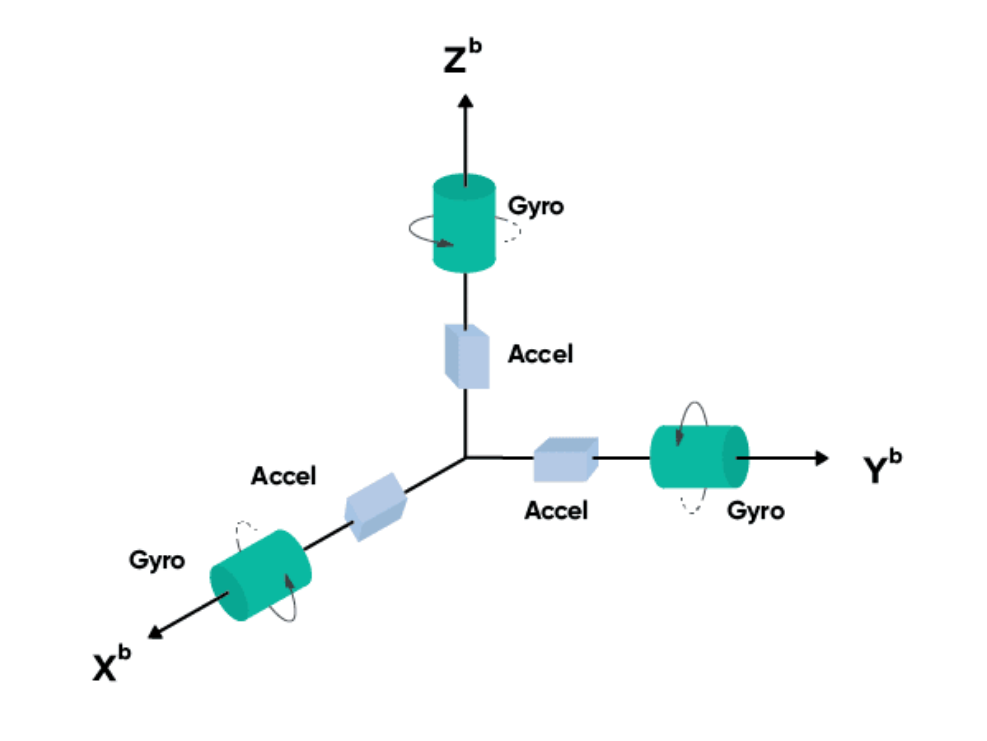
\includegraphics[width=0.5\linewidth]{../imagenes_marco_teorico/giroscopio_ejes.png}
    \caption{Se observa el tipo de dato obtenido de una IMU. Para cada eje, la aceleración y rotación correspondiente. Imagen extraída de \cite{advancednavigation_imu_intro}}
\end{figure}

Se clasifican en cuatro grados según su precisión \cite{10814674}: para consumo, de uso industrial, de uso táctico, y para navegación. Los de menor grado se basan en sistemas micro-electromecánicos que miden la aceleración lineal y angular según el movimiento de masas suspendidas. En este sistema hay dos componentes principales: el acelerómetro y el giróscopo. 

\begin{figure}[H]
    \centering
    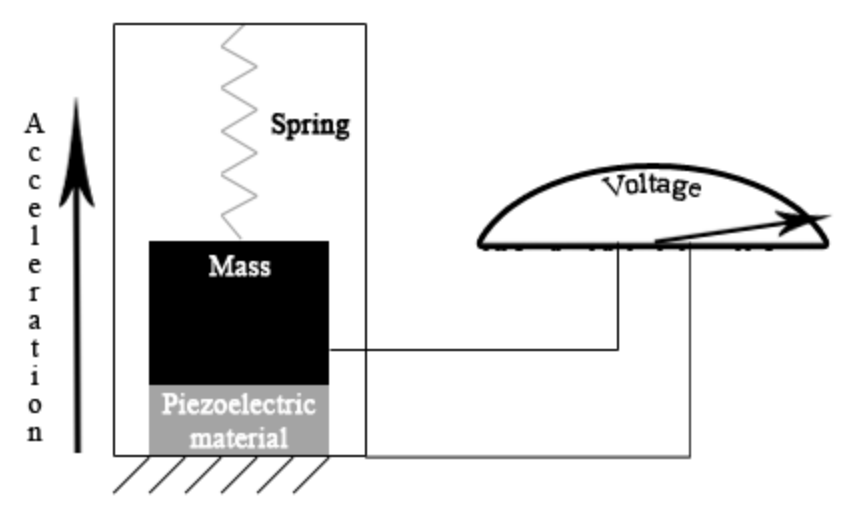
\includegraphics[width=0.8\linewidth]{../imagenes_marco_teorico/modelo_acelerometro_resorte.png}
    \caption{Modelo de acelerómetro para un eje particular. Imagen extraída de \cite{toniK_accelerometer_basics}.}
    \label{fig:acelerometro}
\end{figure}

En un acelerómetro, para cada eje hay una masa suspendida conectada a un resorte. Al percibir una aceleración en el eje correspondiente, en el caso de \ref{fig:acelerometro} hacia la parte superior de la imagen, por inercia la masa ejercerá presión sobre un material piezoeléctrico, el cual generará un voltaje proporcional a la presión recibida, el cual será traducido posteriormente a una medida de aceleración.

\begin{figure}[H]
    \centering
    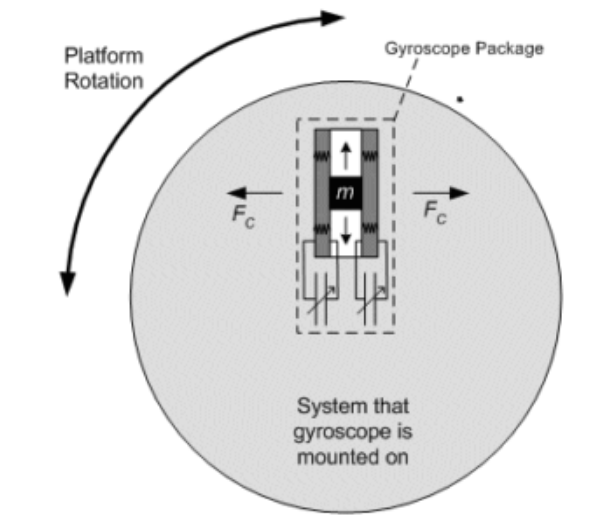
\includegraphics[width=0.5\linewidth]{../imagenes_marco_teorico/modelo_giroscopo.png}
    \caption{Modelo de un giróscopo en un eje particular. Imagen extraída de \cite{ericco2019memsgyro}.}
    \label{fig:giroscopio}
\end{figure}

En un giróscopo, una de las formas de medir la velocidad angular consiste en utilizar una masa suspendida para cada eje, a la cual se le induce una vibración continua. Debido al efecto Coriolis, cuando existe una rotación alrededor del eje correspondiente aparece una fuerza sobre la masa vibrante, perpendicular a su dirección de movimiento.

Esta fuerza provoca un pequeño desplazamiento lateral de la masa, lo que genera una diferencia de capacitancia entre electrodos ubicados a los lados del sensor. Dicha variación capacitiva se traduce en una señal eléctrica que puede utilizarse para estimar la velocidad angular del sistema.

En el caso de la Figura \ref{fig:giroscopio}, si hubiera una rotación en sentido horario y la masa estuviera vibrando de abajo hacia arriba, es decir, desde el centro hacia el borde, se produciría una fuerza lateral hacia la izquierda.



Los sistemas inerciales de menor grado son los más accesibles, pero sus sesgos crecen rápido, degenerando la integración de la pose en pocos segundos. Los de mayor grado poseen, además, giróscopos de fibra óptica, que miden el ratio angular enviando dos rayos de luz. Los mismos viajan en direcciones opuestas a través de un círculo de fibra óptica y vuelven a un sensor. De no haber rotación, volverían al mismo tiempo, y de haber, cambiaría el tiempo de alguno de los dos siguiendo el efecto Sagnac \cite{canalgeomatics_fiberopticgyros}.

\begin{table}[H]
\centering
\caption{Clasificación de IMUs según el sesgo del giróscopo y sus aplicaciones típicas.}
\label{tab:sesgos_imu}
\begin{tabular}{l c p{7cm}}
\toprule
\textbf{Grado} & \textbf{Sesgo del giróscopo (°/h)} & \textbf{Aplicaciones} \\
\midrule
Consumo      & $> 10$           & Teléfonos celulares, relojes inteligentes, controles de videojuegos \\
Industrial   & $1$ -- $10$       & Drones, robótica móvil, automoción \\
Táctico      & $0.1$ -- $1$      & UAVs, sistemas de defensa, instrumentación industrial de precisión \\
Navegación   & $< 0.01$          & Aeroespacial, submarinos, navegación inercial de alta precisión \\
\bottomrule
\end{tabular}
\end{table} 

\subsection{Cinemática de la IMU}

Para modelar el comportamiento de los sensores, se describe su cinemática en \cite{LeuteneggerLynenBosseSiegwartFurgale2015} del siguiente modo:

Sea $\mb{C}_{AB}$ la matriz de rotación de $B$ a $A$, $\mb{\rho}$ la posición, $\mb{q}$ la rotación, $\mb{v}$ la velocidad, ${}_ca_b$ el vector $a$ de $b$ expresado en el sistema de referencia $c$, $\mb{a}$ la aceleración, $\mb{b}_a, \mb{b}_g$ los sesgos del acelerómetro y giróscopo. Asumiendo que la rotación de la Tierra es despreciable respecto a las medidas del giroscopio, tenemos el modelo no lineal:

\begin{equation}
\begin{aligned}
{}_{w}\dot{\mathbf{\rho}}_{s} &= \mathbf{C}_{ws}\,{}_{s}\mathbf{v}, \\[4pt]
%
\dot{\mathbf{q}}_{ws} &= \frac{1}{2}\,\boldsymbol{\Omega}\!\left({}_{s}\boldsymbol{\omega}\right)\,\mathbf{q}_{ws}, \\[6pt]
%
{}_{s}\dot{\mathbf{v}} &=
{}_{s}\tilde{\mathbf{a}}
+ \mathbf{w}_{a}
- \mathbf{b}_{a}
+ \mathbf{C}_{sw}\,{}_{w}\mathbf{g}
- \left({}_{s}\boldsymbol{\omega}\right) \times {}_{s}\mathbf{v}, \\[6pt]
%
\dot{\mathbf{b}}_{g} &= \mathbf{w}_{b_g}, \\[4pt]
%
\dot{\mathbf{b}}_{a} &= -\frac{1}{\tau}\,\mathbf{b}_{a} + \mathbf{w}_{b_a}.
\label{imu_formula}
\end{aligned}
\end{equation}


con $\mathbf{w}_i$ ruidos gaussianos de media cero y la matriz $\Omega$ formada por el ratio angular estimado ${}_s\omega = {}_s\tilde{\omega} + \mathbf{w}_g - \mathbf{b}_g$ a partir de la medida ${}_s\tilde{\omega}$. En esta formulación, la actualización del cuaternión se interpreta como una perturbación a izquierda:

\[
\Omega({}_s\omega)\,\mathbf{q}_{ws} = \mathbf{q}_{ws} \oplus_{\mathrm{izq}} {}_s\boldsymbol{\omega}.
\]

Se usa esta convención porque la cinemática está escrita en el marco del sensor y el término incremental se aplica por pre-multiplicación.

La primera ecuación describe la evolución de la posición del sensor $s$ en coordenadas globales $w$, dada por la velocidad expresada en el marco del sensor multiplicada por un cambio de base que lleva su rotación al marco global.

La segunda ecuación describe la evolución de la rotación, expresada en cuaterniones, como la suma en el grupo $SO(3)$ de la rotación y la estimación del ratio angular medido.

La tercera ecuación describe la evolución de la velocidad, es decir la aceleración, en el marco del sensor. Comienza con la aceleración medida, a la cual se le suma un ruido gaussiano del acelerómetro. Este ruido surge inherentemente al modelar sensores. Por otro lado, se le resta el sesgo del acelerómetro y se le suma la gravedad rotada a las coordenadas del sensor. Finalmente, se le resta el producto cruz entre el ratio angular estimado del sensor y su velocidad, como corrección del efecto Coriolis.

La cuarta ecuación describe la evolución del sesgo del giroscopio como un ruido gaussiano de media cero, mientras que la quinta ecuación describe la evolución del sesgo del acelerómetro como un ruido gaussiano también, aunque compensado por una fuerza que tiende a mantenerlo alrededor del cero a partir de una constante temporal $\tau > 0$.

Notemos que, al modelar ambos ruidos con variables aleatorias, nos encontramos con lo que se conoce como camino aleatorio y camino aleatorio acotado, respectivamente. Este comportamiento los hace difíciles de controlar, y provoca que un sistema de estimación de la pose basado exclusivamente en las mediciones inerciales tienda a degenerarse a medida que pasa el tiempo. Para contrarrestar este fenómeno, se hace lo siguiente:

Al iniciar el robot, se lo deja quieto unos segundos. Luego, se toma el promedio de las mediciones de aceleración y rotación, y se las considera el sesgo a restar. Esta estimación permite una inicialización razonable del sistema, pero la evolución temporal la hará inestable. Para contrarrestarlo, es necesario correlacionar los datos con los de otros sensores. Históricamente, los filtros de Kalman \cite{MasnadiShirazi2019KalmanTutorial} constituyen una técnica muy empleada para fusionar los distintos sensores a partir de matrices, pero en el marco de este trabajo no es factible. Esto se debe a que el modelo que empleamos es no lineal, se basa en algoritmos iterativos de optimización con derivadas, y que el gran número de gaussianas da lugar a demasiados parámetros a optimizar. De este modo, el sesgo se corrige mediante algoritmos de optimización que fusionan los datos visuales con los inerciales.